\documentclass[12pt, letterpaper, fleqn]{article}
\usepackage[letterpaper, margin=.75in]{geometry}
\usepackage[utf8]{inputenc}
\usepackage{amsmath}
\usepackage{amssymb}
\usepackage{algorithmicx}
\usepackage{algpseudocode}
\usepackage{algorithm}
\usepackage[english]{babel}
\usepackage{amsthm}
\usepackage{graphicx}
\usepackage{xcolor}
\graphicspath{ {.} }
\usepackage{fancyhdr}
\usepackage{tikz}
\usepackage{hyperref}
\usepackage{cancel}
\newcommand*\circled[1]{\tikz[baseline=(char.base)]{
            \node[shape=circle,draw,inner sep=2pt] (char) {#1};}}
\setlength\parindent{0pt}
\def\join{\mathbin{\ojoin\mkern0mu\bowtie\mkern3mu\ojoin}}

%\pagestyle{fancy}
%\fancyhf{}
%\rhead{Bill Yang}
%\renewcommand{\headrulewidth}{0pt}

\newcommand{\handout}[5]{
   \renewcommand{\thepage}{#1-\arabic{page}}
   \noindent
   \begin{center}
   \framebox{
      \vbox{
%    \hbox to 5.78in { {\bf M328K Number Theory} \hfill #2 }
%       \vspace{4mm}
%       \hbox to 5.78in { {\Large \hfill #5  \hfill} }
%       \vspace{2mm}
%       \hbox to 5.78in { {\it #3 \hfill #4} }
    \hbox to 5.78in { { Bill Yang} \hfill {Due: #2} }
       \vspace{4mm}
       \hbox to 5.78in { {\Large \hfill #5  \hfill} }
       \vspace{2mm}
       \hbox to 5.78in { {#3 \hfill #4} }
      }
   }
   \end{center}
   \vspace*{4mm}
}

\newcommand{\ho}[5]{\handout{#1}{#2}{#3}{Instructor: #4}{Homework #1}}

\begin{document}
  \ho{10}{5/1/20}{CS386D Database Systems}{Daniel Miranker} \\

  \section{Part 1}
\begin{center}
\begin{tabular} { | c | c | c | c |}
  \hline  
  Client Location & Server Location & Load Time (seconds) & Bytes/second \\
  \hline
  Local Machine & Local Machine & 115.4 & 11.1 Mbytes / second \\
  \hline
  Local Machine & AWS & 95096.3 & 13.9 Kbytes / second \\
  \hline
  AWS & AWS & 153.9 & 8.3 Mbytes/ second \\
  \hline


\end{tabular}
\end{center}


  \section{Part 2}
  \textbf{10.}\\
  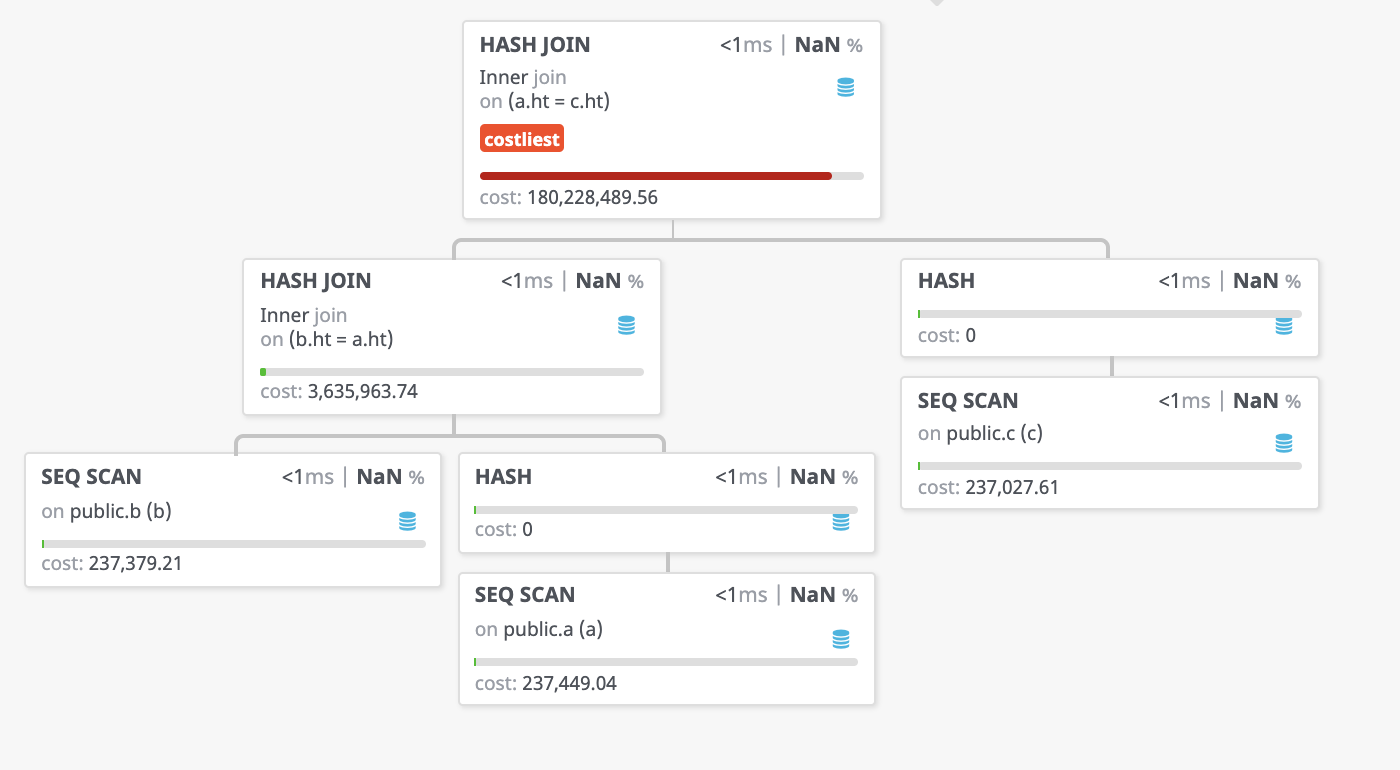
\includegraphics[scale=0.5]{query_pics/10.png} \\

  \textbf{11.}\\
  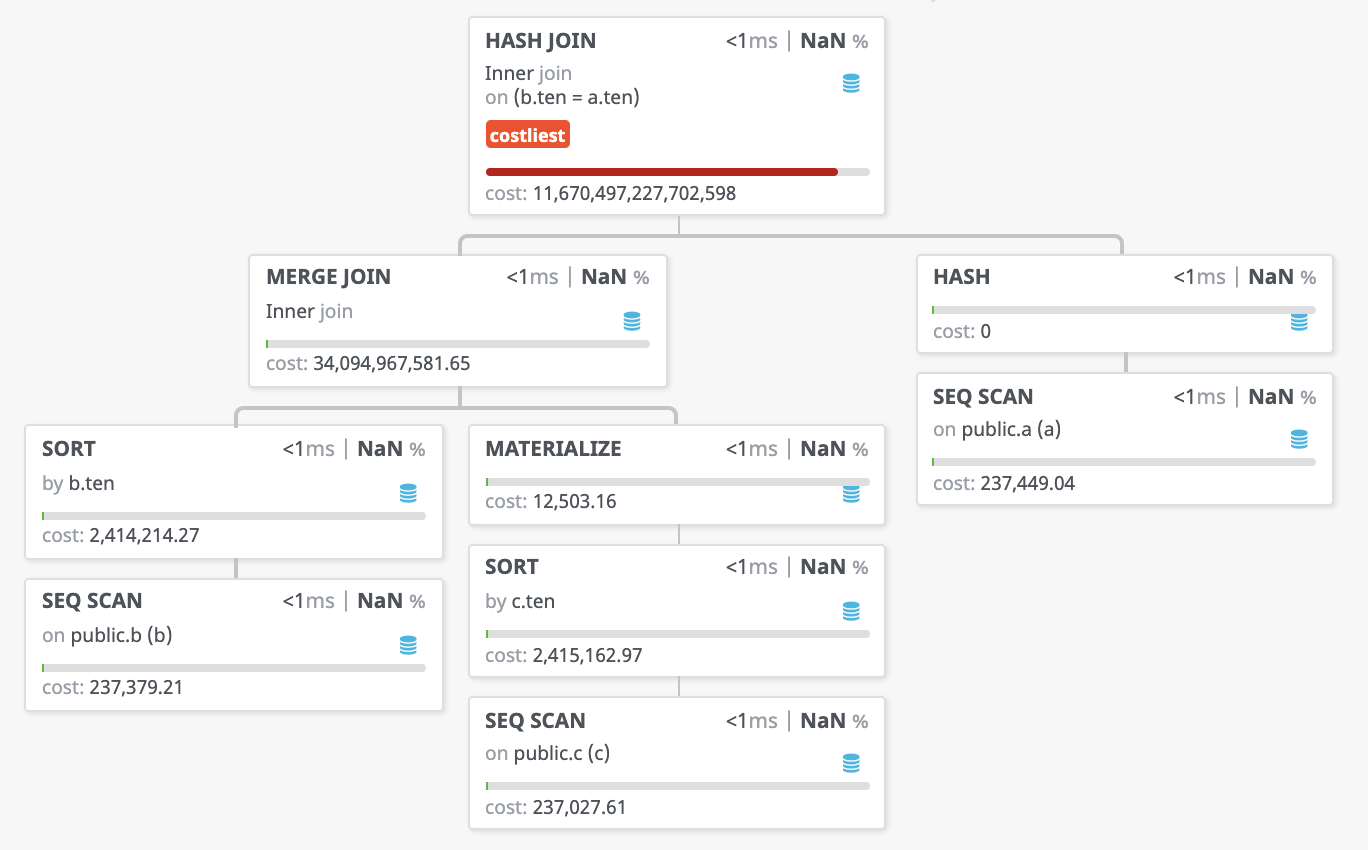
\includegraphics[scale=0.5]{query_pics/11.png} \\

  \textbf{12.} \\
  A.hund = B.hund = C.hund and A.ot = B.ot = C.ot is the threshold. \\
  ot produces the same result as ht \\
  hund produces the same result as ten \\

  \textbf{13.}\\
  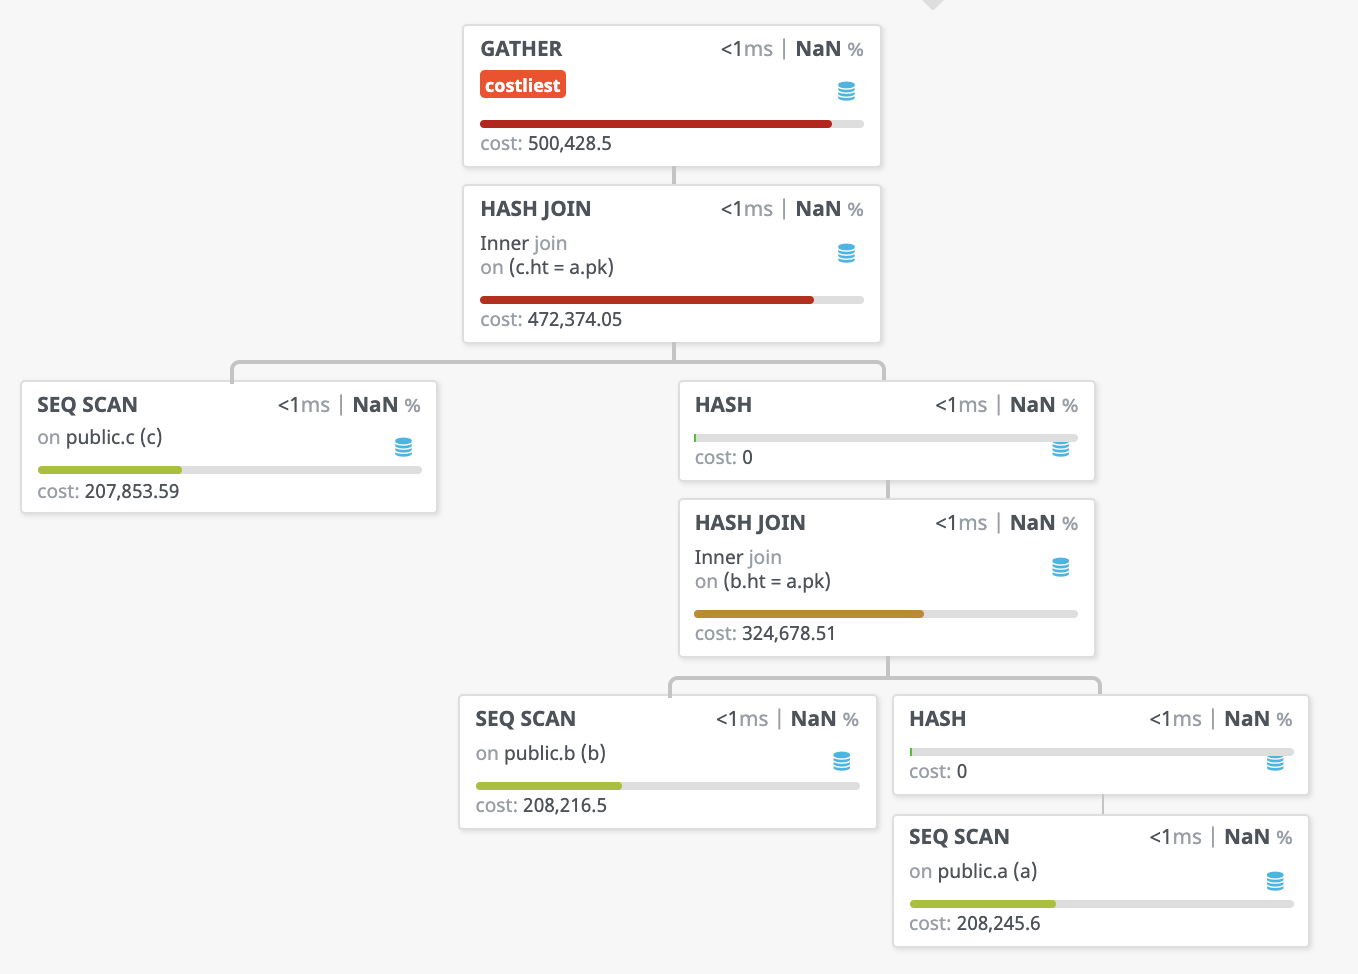
\includegraphics[scale=0.5]{query_pics/13.png} \\

  \textbf{14.}\\
  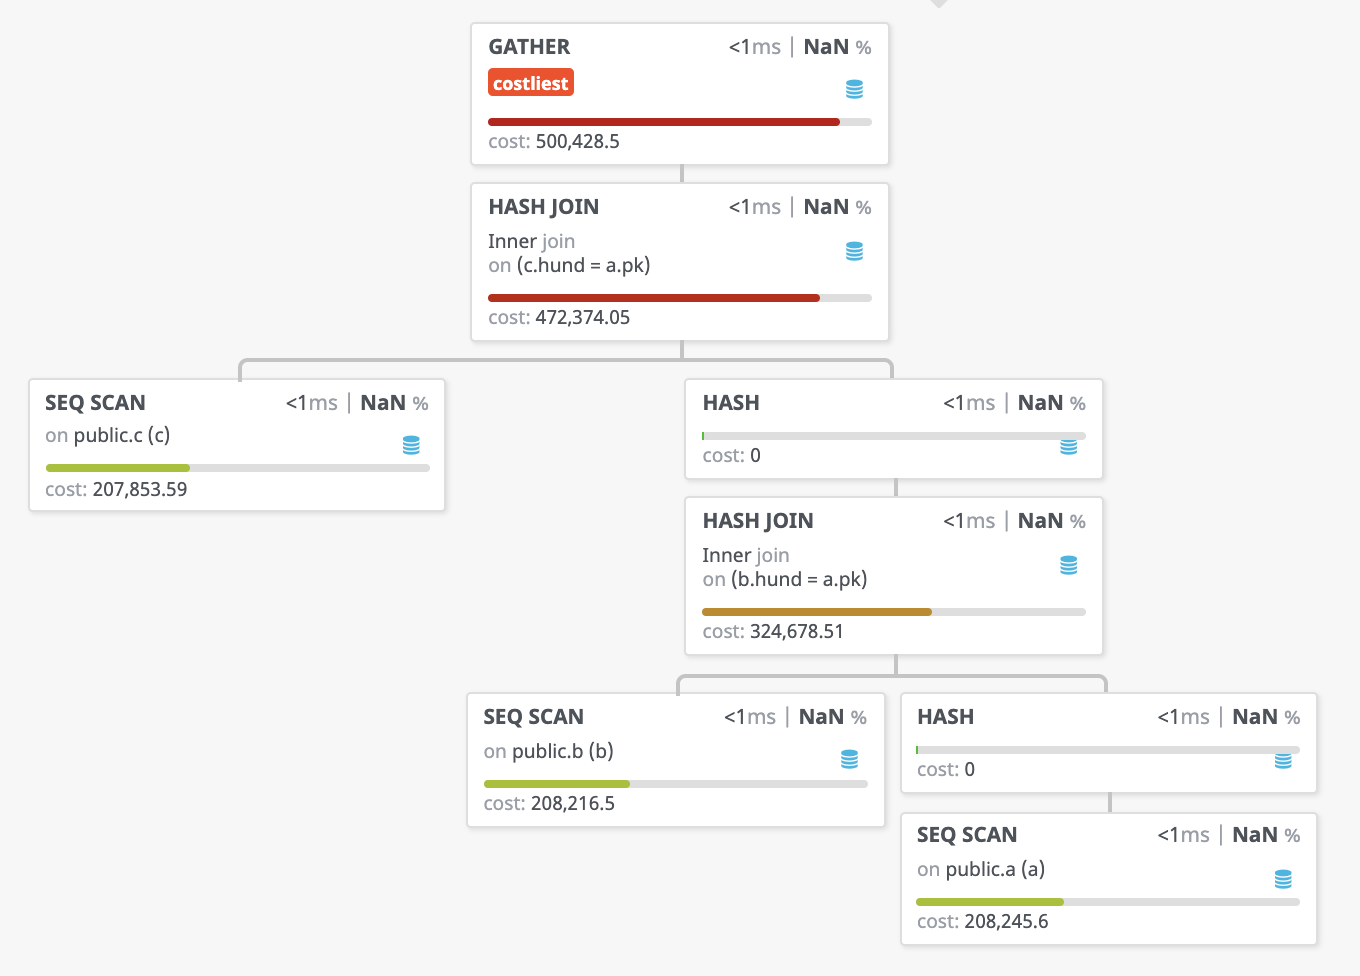
\includegraphics[scale=0.5]{query_pics/14.png} \\

  \textbf{15.} \\
  13 and 14 produce the same plan. \\

  \textbf{16.}\\
  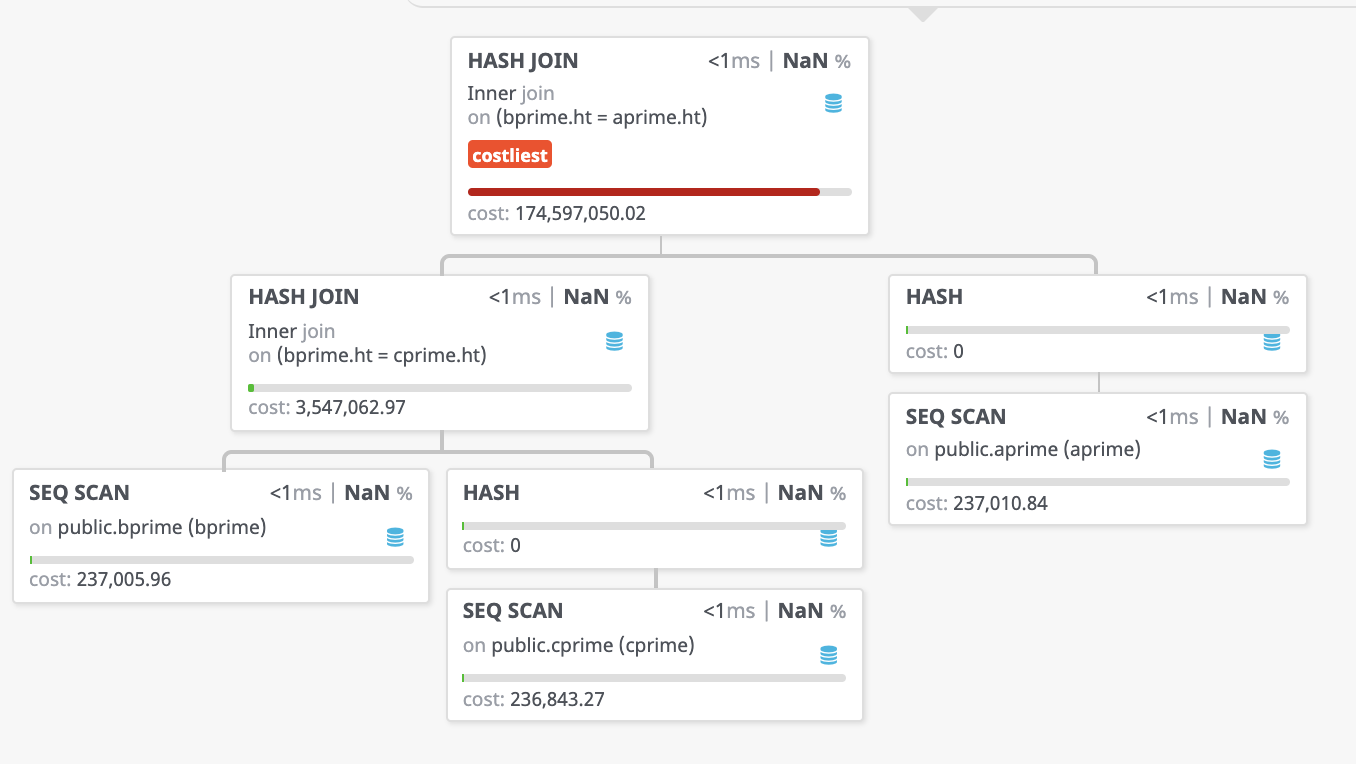
\includegraphics[scale=0.5]{query_pics/16.png} \\

  \textbf{17.}\\
  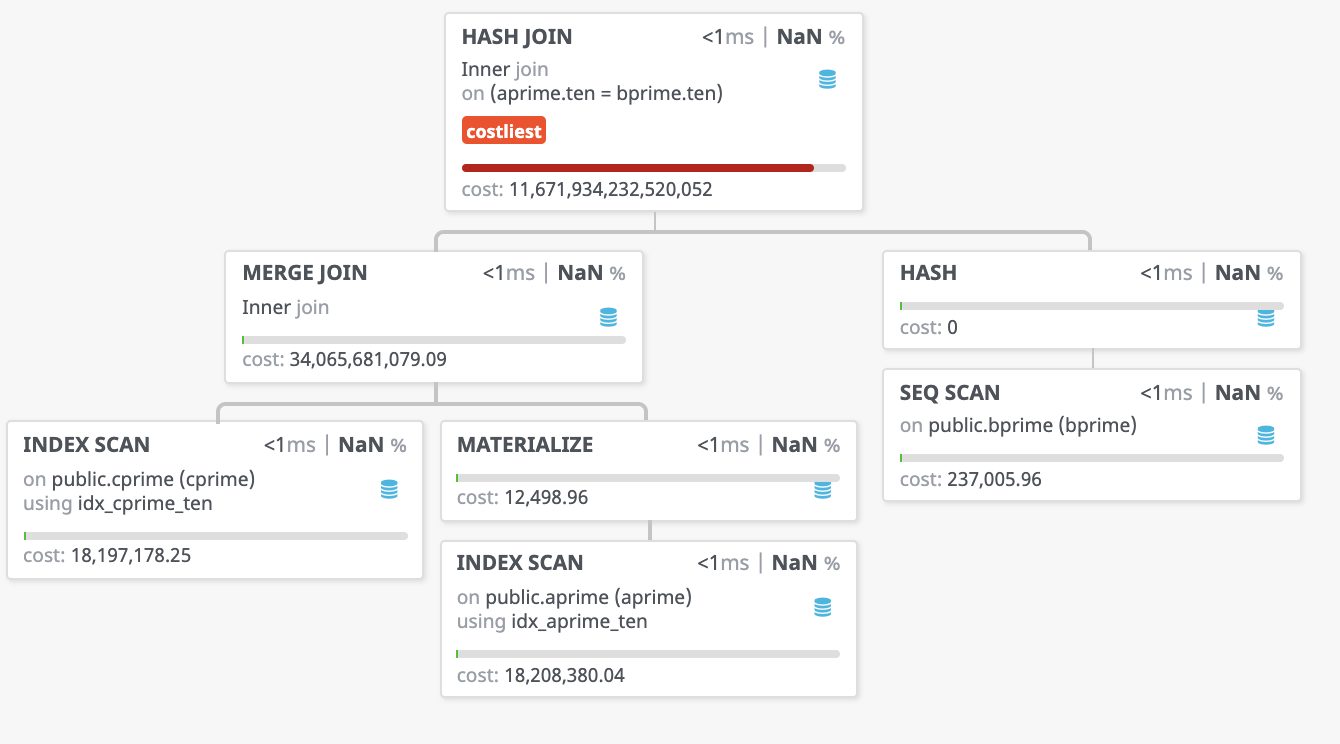
\includegraphics[scale=0.5]{query_pics/17.png} \\

  \textbf{18.} \\
  A.hund = B.hund = C.hund and A.ot = B.ot = C.ot is the threshold. \\
  ot produces the same result as ht \\
  hund produces the same result as ten \\

  \textbf{19.}\\
  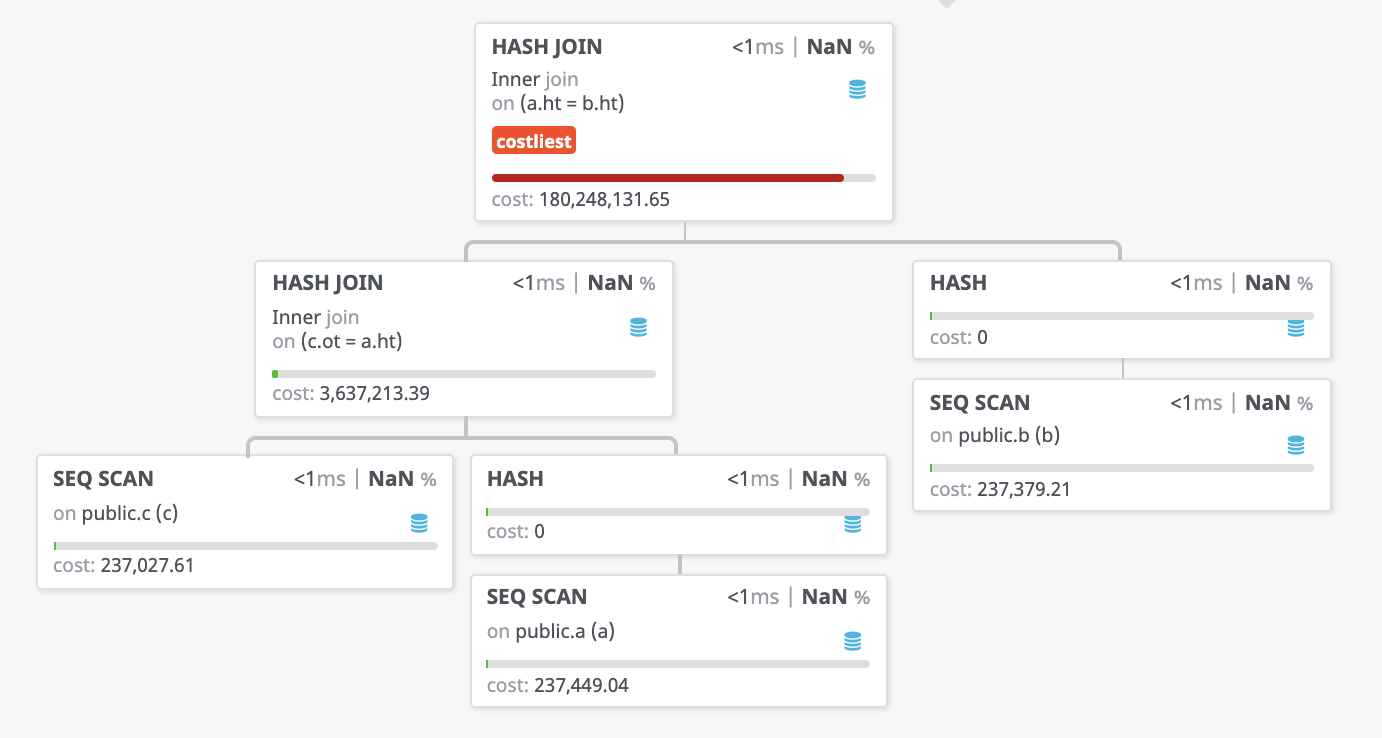
\includegraphics[scale=0.5]{query_pics/19.png} \\
  
  \textbf{20.}\\
  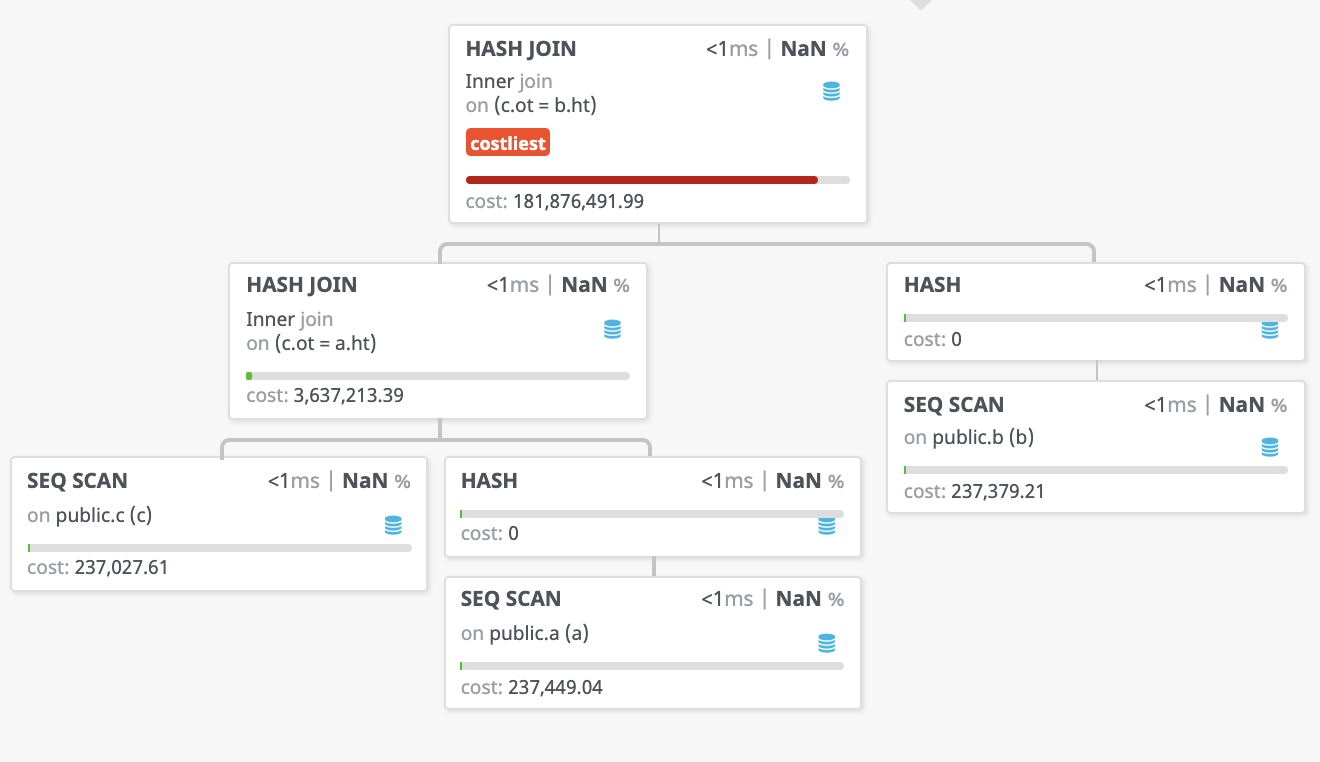
\includegraphics[scale=0.5]{query_pics/20.png} \\

  \textbf{21.}\\
  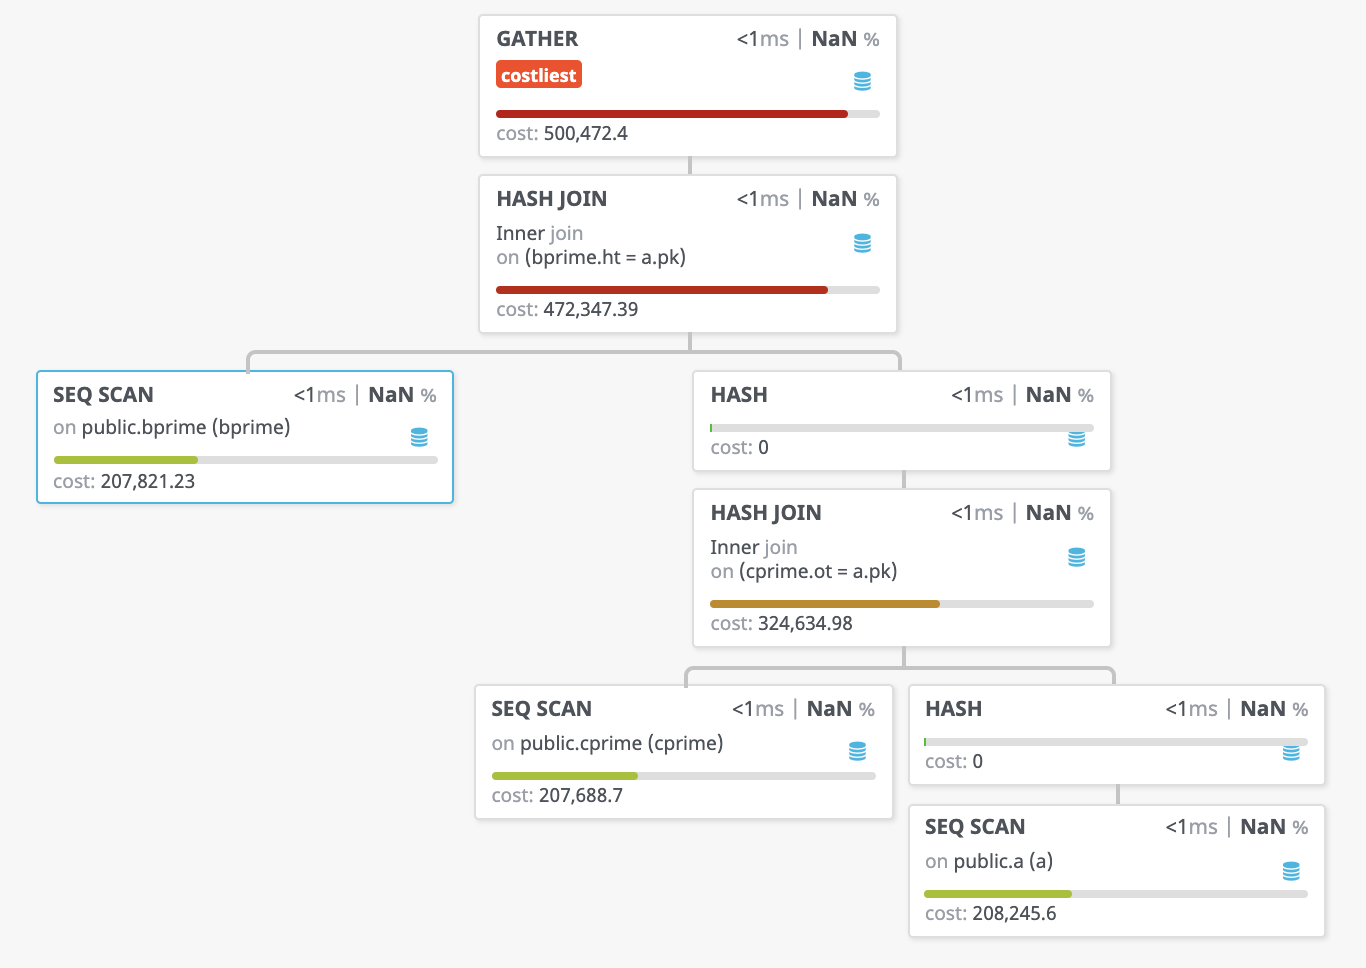
\includegraphics[scale=0.5]{query_pics/21.png} \\

  \textbf{22.}\\
  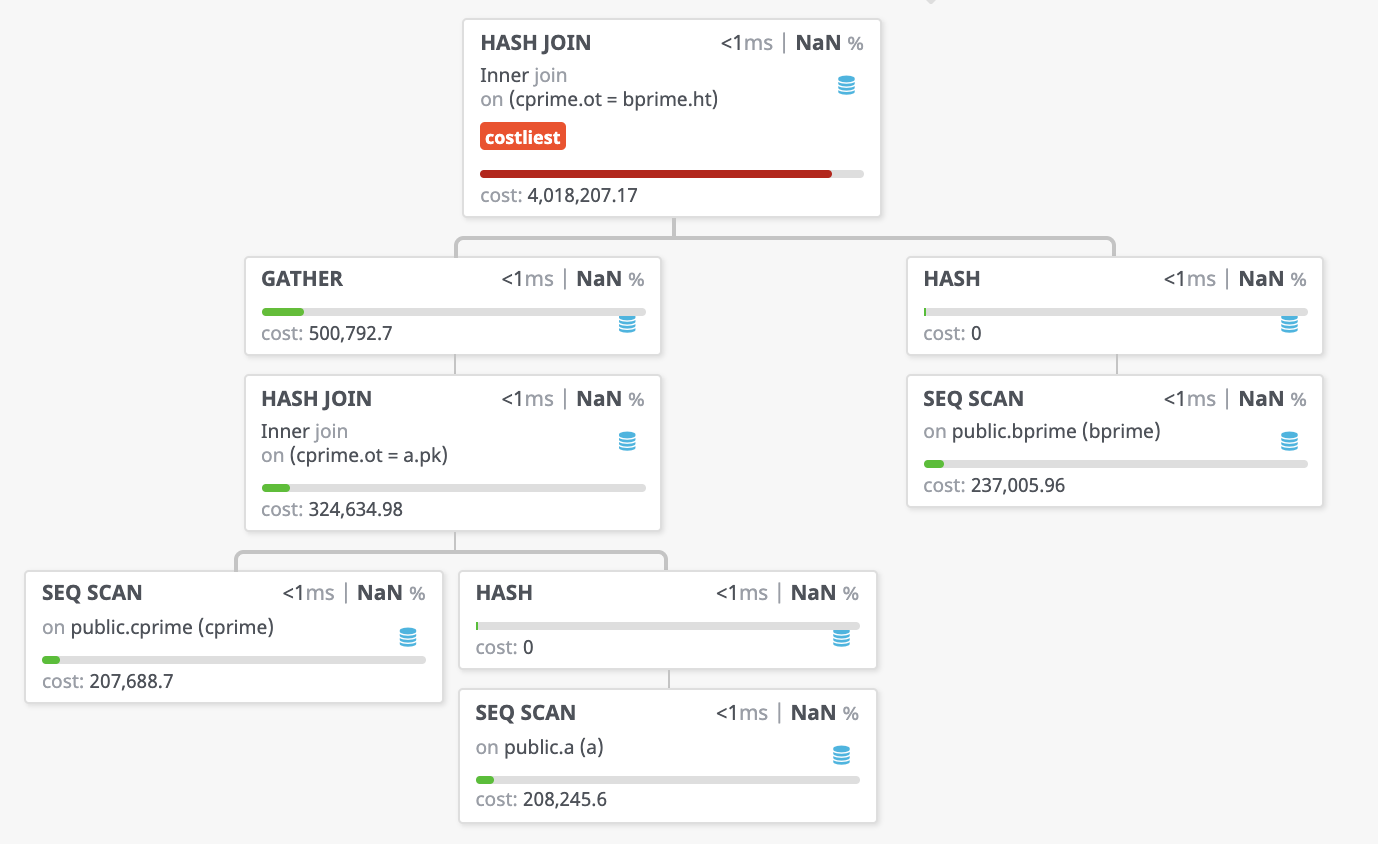
\includegraphics[scale=0.5]{query_pics/22.png} \\

  The join order was not affected in the non-indexed tables. The optimizer did
  the same thing regardless of how I wrote the query. In the queries with the
  indexed tables, the join order was affected by how I wrote the query for the
  three way join.

  \section{Part 3: Datalog Syntax}
  \textbf{1.} \\
  Triggers, and Views\\

  \textbf{2.} \\
  AI (Knowledge based Systems), Enterprise Information Integration, and Business
  Process Execution Language.\\

  \textbf{3. }\\
  $\pi_{Person} ((Frequents \join Likes) \join Sells)$\\

  \textbf{4.} \\
  a) Sells  = 3\\
  b) Happy = 1\\
  c) Likes = 2 \\

  \textbf{5.} \\
  bar, beer, p\\

  \textbf{6.} \\
  a) 5 subgoals \\
  b) 1 distinguished variable\\

  \textbf{7.} \\
  a) OpenDays(r,d) = Restaurant(r, d) \\
  b) ClosedDays(r,d) = Restaurant(r) and Restaurant(\_, d) and not Restaurant(r, d)\\
  c) no\\
  d) it cannot be concluded that it is closed.\\

  \textbf{8.} \\
  a) unsafe: price \\
  b) unsafe: r2, d2, o2, c2\\
  c) safe




\end{document}
